Reazioni in cui mettiamo a reagire un acido e una base.
\subsection{Esempi}
\ce{HCl(aq) + NH_3(aq) <--> NH_4^+(aq) + Cl^-(aq)}

\vspace{0.2cm}(Nota: sia accanto all'acido cloridrico che all'ammoniaca c'è scritto acquoso (aq), perché entrambe le specie sono gas. Noi li facciamo gorgogliare in acqua, ottenendo delle soluzioni acquose dell'acido e della base. Stiamo quindi immaginando di avere due soluzioni acquose che mescoleremo insieme)

Questa reazione produce lo ione $\rm NH_4^+$, in quanto l'acido cloridico è un acido forte, totalmente dissociato, quindi con $\rm HCl(aq)$ intendiamo ione $\rm H^+$ e ione $\rm Cl^-$; non è così invece per l'ammoniaca che è una base debole. Lo ione $\rm H^+$ dell'HCl, già dissociato, protona l'ammoniaca grazie al doppietto presente sull'azoto dell'$\rm NH_3$ (infatti tale doppietto è adatto a legare questo ulteriore protone), formando lo ione $\rm NH_4^+$, mentre dall'HCl resta lo ione cloruro $\rm Cl^-$.

Questa è una reazione acido-base, per cui si forma un sale che è il cloruro di ammonio, il quale in acqua, come tutti gli elettroliti forti, è totalmente dissociato, infatti nella reazione c'è una singola freccia. Va poi da ricordare che tutti i sali sono elettroliti forti per definizione.

\vspace{0.2cm}\ce{CH_3COOH + H_2O(l) <--> CH_3COO^- + H_3O^+(aq)}

\vspace{0.2cm}L'acido acetico in acqua si dissocia, liberando un protone che si somma all'acqua usando il doppietto dell'ossigeno disponibile per legarlo, formando lo ione $\rm H_3O^+$. Dell'acido resterà lo ione acetato $\rm CH_3COO^-$.

Questa reazione non è tutta spostata verso destra, per cui mettiamo le doppie frecce. Infatti questa seconda reazione è la dissociazione di un acido debole.

\vspace{0.2cm}\ce{CH_3COOH + HClO_4(aq) <--> CH_3COOH_2^+(aq) + ClO_4^-(aq)}

\vspace{0.2cm}In questa terza reazione abbiamo due acidi: acido acetico e acido perclorico. Abbiamo visto che ci sono speci anfotere, cioè che si comportano o da acido o da base a seconda del partner. Da un punto di vista formale allora, possiamo "forzare la mano" e scegliere una specie etichettata acida per dimostrare che anch'essa può comportarsi da base se in presenza di un acido estremamente più forte: sebbene l'acido acetico sia un acido, se è in soluzione con un acido molto più forte (l'acido perclorico è l'acido più forte che esista) anziché dissociarsi cedendo un protone e rimanendo ione acetato vedrà l'$\rm HClO_4$ cedere un protone, formando lo ione $\rm ClO_4^-$. Questo protone si somma all'acido acetico ottenendo la specie $\rm CH_3COOH_2^+$, ione acidioacetato. Quindi in questa reazione, avendo forzato molto, l'acido acetico si è comportato da base, perché ha accettato il protone.

Attenzione! Ciò non implica che l'acido acetico sia un afolita. Questo esempio serve solo a far vedere come non potremmo dire in assoluto che specie sia acida o basica se prima non vediamo quale sia il partner, visto che stiamo parlando di reazioni acido-base: se è messo in acqua, l'acido acetico si comporta da acido, se è messo in una soluzione di acido perclorico si comporta da base.

\vspace{0.2cm}Vediamo ora altre reazioni

\begin{center}
    \begin{tabular}{llllllll}
        \textbf{Nome} & \textbf{Acido 1} & & \textbf{Base 2} & & \textbf{Base 1} & & \textbf{Acido 2}\\[0.3ex]
        Acido cloridico & HCl & + & $\rm H_2O$ & \ce{<-->} & $\rm Cl^-$ & + & $\rm H_3O^+$\\[0.3ex]
        Acido nitrico & $\rm HNO_3$ & + & $\rm H_2O$ & \ce{<-->} & $\rm NO_3^-$ & + & $\rm H_3O^+$\\[0.3ex]
        Acido carbonico & $\rm H_2CO_3$ & + & $\rm H_2O$ & \ce{<-->} & $\rm HCO_3^-$ & + & $\rm H_3O^+$\\[0.3ex]
        Acido acetico & $\rm CH_3CO_2H$ & + & $\rm H_2O$ & \ce{<-->} & $\rm CH_3CO_2^-$ & + & $\rm H_3O^+$\\[0.3ex]
        Acido cianidrico & $\rm HCN$ & + & $\rm H_2O$ & \ce{<-->} & $\rm CN^-$ & + & $\rm H_3O^+$\\[0.3ex]
        Acido solfidrico & $\rm H_2S$ & + & $\rm H_2O$ & \ce{<-->} & $\rm HS^-$ & + & $\rm H_3O^+$\\[0.3ex]
        Ammoniaca & $\rm H_2O$ & + & $\rm NH_3$ & \ce{<-->} & $\rm OH^-$ & + & $\rm NH_4^+$\\[0.3ex]
        Ione carbonato & $\rm H_2O$ & + & $\rm CO_3^{2-}$ & \ce{<-->} & $\rm OH^-$ & + & $\rm HCO_3^-$\\[0.3ex]
        Acqua & $\rm H_2O$ & + & $\rm H_2O$ & \ce{<-->} & $\rm OH^-$ & + & $\rm H_3O^+$\\[0.3ex]
    \end{tabular}
\end{center}

Nelle reazioni ci devono essere almeno due partner, perché non esiste un acido se non c'è una base, cioè se una specie cede protoni è indispensabile che ci sia un'altra specie che li acquisti, quindi sia a sinistra che a destra della reazione devono esserci almeno due composti.

Nelle prime sei reazioni l'acqua si comporta da base, acquistando un protone e diventando ione $\rm H_3O^+$, specie che a sua volta potrà cedere un protone, quindi è un acido. Chiaramente lo ione che resta dalla dissociazione dell'acido sarà la base coniugata.

Nelle due successive l'acqua è in presenza di basi, per cui si comporta da acido, dunque sarà la specie che cede il protone, dando lo ione $\rm OH^-$ in soluzione che è la base coniugata.

Nell'ultima reazione vediamo che due molecole d'acqua danno luogo ad uno ione $\rm H_3O^+$ e ad uno ione $\rm OH^-$. Approfondiremo.
\subsection{Sistemi acido-base secondo Brönsted}
Per generalizzare il comportamento che abbiamo descritto non possiamo parlare di acido o di base, ma di sistemi acido-base.

Dato che gli acidi cedono protoni, li etichettiamo con H-A e con $\rm H^+$ indichiamo il protone e con $\rm A^-$ ciò che resta. Etichettiamo invece con B la base, che sarà tale se e solo potrà acquistare il protone:

\begin{figure}[H]
    \centering
    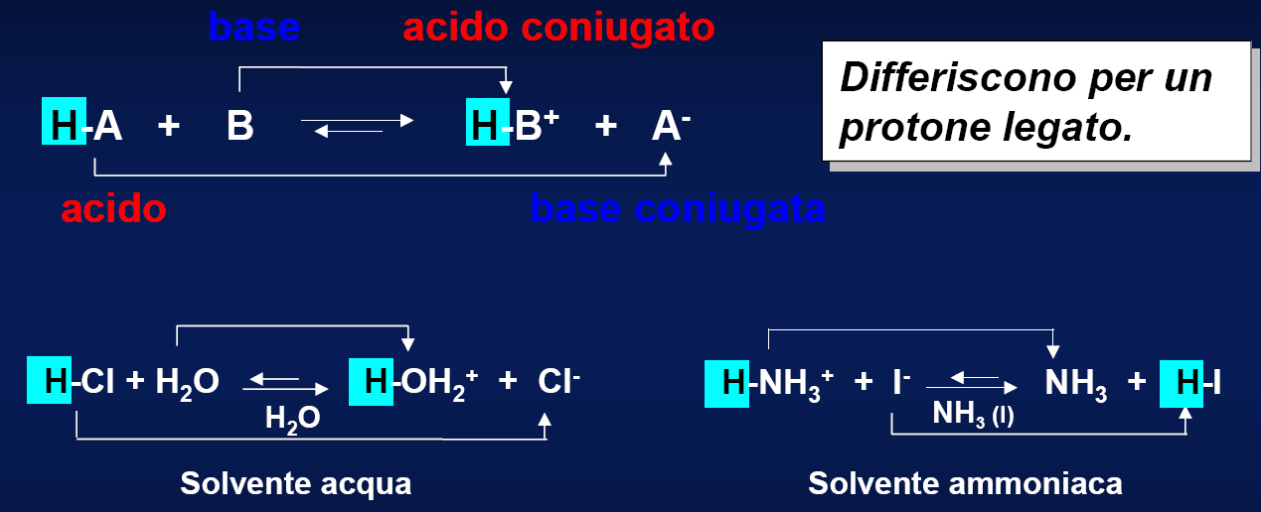
\includegraphics[width=12cm]{immagini/acido_base_coniugata.png}
\end{figure}

Con questo simbolismo quindi avremo sempre a sinistra un acido e una base, mentre a destra avremo la base coniugata dell'acido e l'acido coniugato della base, cioè a sinistra avremo le speci che vogliamo far reagire e a destra le loro speci coniugate.

Va da notare che la differenza tra speci coniugate è di un protone: $\rm H-A$ e $\rm A^-$ differiscono per un protone, così come B e $\rm B^+$.

\vspace{0.2cm}\textbf{ES.1}
\begin{figure}[H]
    \centering
    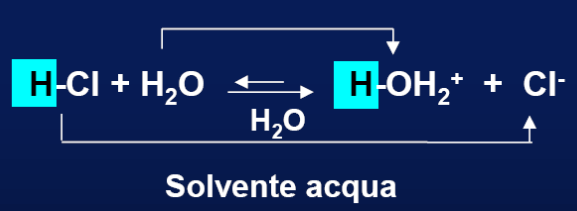
\includegraphics[width=6cm]{immagini/acido_base_coniugata_es1.png}
\end{figure}

HCl è l'acido, $\rm Cl^-$ è la base coniugata, la quale vi differisce per un protone.

$\rm H_2O$ accetterà questo protone e quindi sarà una base mentre il suo acido coniugato è $\rm H_3O^+$, da cui differisce per un protone.

\vspace{0.2cm}\textbf{ES.2}
\begin{figure}[H]
    \centering
    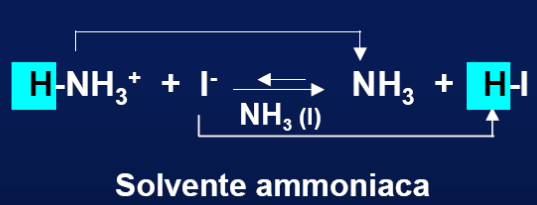
\includegraphics[width=6cm]{immagini/acido_base_coniugata_es2.png}
\end{figure}

Qui come reagenti abbiamo ione ammonio e ione ioduro.

Lo ione ammonio ha un protone in più rispetto all'ammoniaca, il quale può essere ceduto. Quindi l'$\rm NH_4^+$ è un acido e la sua base coniugata è l'$\rm NH_3$.

Se lo ione ammonio cede un protone, serve una base che lo accetti: lo ione ioduro $\rm I^-$, che accetta il protone diventando acido iodidrico HI, che sarà l'acido coniugato.

Tra l'altro questa reazione non avviene in acqua: il solvente è l'ammoniaca che sarà in eccesso.

Ancora una volta ribadiamo quindi che non si può parlare di acidi e basi, ma di sistemi acido-base.

\vspace{0.2cm}Facciamo adesso un ripasso della differenza tra speci forti e deboli:

\begin{itemize}
    \item \textbf{Acidi forti}: si dissociano totalmente
    
    ES: \ce{HCl + H_2O -> H_3O^+ + Cl^-}
    \item \textbf{Basi forti}: si dissociano totalmente
    
    ES: \ce{KOH -> K^+ + OH^-}
    \item \textbf{Acidi deboli}: non si dissociano del tutto
    
    ES: \ce{CH_3CO_2H <--> H^+ + CH_3CO_2^-}
    \item \textbf{Basi deboli}: non si dissociano del tutto
    
    ES: \ce{NH_3 + H_2O <--> NH_4^+ + OH^-}
\end{itemize}

Per poter valutare se una specie sia forte o debole, cioè se sia totalmente o parzialmente dissociata, dobbiamo andare a verificare il valore della costante di equilibrio. Se essa ha un valore piccolo significa che c'è stata poca dissociazione, fatto indicato dalla doppia freccia nelle reazioni. Se invece ha un valore grande allora la specie chimica sarà totalente dissociata.

\vspace{0.2cm}Vediamo le costanti di dissocazione per i casi deboli, che si calcolano come il rapporto tra il prodotto della concentrazione dei prodotti elevate ciascuna per il proprio coefficiente stechiometrico e la concentrazione del reagente all'equilibrio elevata per il suo coefficiente stechiometrico:

$$k_a=\rm{\frac{[H^+][CH_3CO_2^-]}{[CH_3CO_2H]}}, \quad [CH_3CO_2H] \neq 0$$

Va da notare che il denominatore è diverso da zero perché all'equilibrio questa specie è ancora largamente indissociata.

Per il caso della base si ha

$$k_b=\rm{\frac{[NH_4^+][OH^-]}{[NH_3]}}, \quad [NH_3]\neq 0$$

In tali espressioni manca la concentrazione dell'acqua, a breve spiegheremo perché.
\subsection{Forza degli acidi e delle basi}
\textbf{ES.}

$$\ce{HCOOH(aq) + H_2O(l) <--> HCOO^-(aq) + H_3O^+(aq)}$$

L'acido formico in acqua dà lo ione formiato, e il protone che si libera si associa all'acqua per formare $\rm H_3O^+$.

Per vedere quanto è avvenuta la dissociazione dobbiamo leggere i valori delle costanti. Ma come otteniamo i valori?

Nei vari esempi che abbiamo visto, partiamo da sistemi neutri e otteniamo degli ioni in soluzione. Sappiamo però che se in soluzione acquosa abbiamo ioni la soluzione condurrà elettricità, solo che i portatori di carica saranno gli ioni anziché gli elettroni. Quindi a partire da misure di conducibilità possiamo risalire alla quantità di ioni che abbiamo in soluzione, ossia possiamo sapere quanto si dissocia una specie chimica tramite misure elettriche.

Per l'esempio di sopra, la costante di dissociazione si potrà scrivere come

$$k= \rm{\frac{[HCOO^-]\cdot[H_3O^+]}{[HCOOH]}} = \frac{\alpha^2}{1- \alpha}\textit{c}$$

Cerchiamo di capire la seconda espressione.

Consideriamo le quantità in gioco prima e dopo la reazione. Se inizialmente abbiamo una mole di acido formico, abbiamo però 0 moli di ione formiato e di $\rm H_3O^+$. Appena la specie si dissocia, avremo $\alpha$ moli per entrambi gli ioni. Ovviamente sarà $\alpha<1$, altrimenti significherebbe che si è dissociato totalmente, quindi all'equilibrio ci saranno $1-\alpha$ moli di reagente. Va da notare che $\alpha$ lo abbiamo già incontrato: è il grado di dissociazione. Ogni molecola di acido che si dissocia produce una molecola di formiato e una di $\rm H_3O^+$, quindi la concentrazione dei prodotti sarà $\alpha^2$, mentre quella dei reagenti $1-\alpha$. Se però non partissimo da una mole, bensì da una concentrazione $c$, ogni quantità andrebbe moltiplicata per $c$. In questo modo avremo $c^2/c$ come fattore, ovvero basta moltiplicare per $c$.

$\alpha$ si ottiene da misure di conducibilità.

In questo modo misuriamo le costanti di dissociazione. Si trova ad esempio

\vspace{0.2cm}$\bullet \rm HClO_4$: $k=10^3$

\vspace{0.2cm}$\bullet \rm HNO_3$: $k=24$

\vspace{0.2cm}$\bullet \rm CH_3COOH$: $k=1.8 \cdot 10^{-5}$

\vspace{0.2cm}$\bullet \rm CH_2ClCOOH$: $k=1.4 \cdot 10^{-3}$

Se nell'acido acetico sostituiamo un idrogeno del gruppo $\rm CH_3$ con un atomo di cloro, il quale è molto elettronegativo, anziché un gruppo $\rm CH_3$ avremo un gruppo $\rm CH_2Cl$. Dato che il cloro è elettronegativo, esso tenderà ad attirare la carica verso questo gruppo, quindi il legame OH, che è quello che si romperà permettendo la dissociazione e quindi la perdita del protone, sarà impoverito di elettroni, quindi romperlo sarà più facile rispetto al caso precedente laddove il cloro manca, quindi la costante cresce.

\vspace{0.2cm}$\bullet \rm CHCl_2COOH$: $k=5 \cdot 10^{-2}$

Se sostituiamo un ulteriore idrogeno con un altro atomo di cloro, avremo il gruppo $\rm CHCl_2$ che comporta un maggiore spostamento di carica verso questo gruppo, quindi un legame OH con meno carica dunque più indebolito. Il protone si libererà più facilmente: la costante cresce.

\vspace{0.2cm}$\bullet \rm CCl_3COOH$: $k=2 \cdot 10^{-1}$

Se sostituiamo tutti e tre gli atomi di idrogeno con tre clori, la costante crescerebbe ancora di più

\vspace{0.2cm}$\bullet \rm HSO_4^-$: $k=10^{-2}$

\vspace{0.2cm}$\bullet \rm NaOH$: $k$ troppo grande

\vspace{0.2cm}$\bullet \rm AgOH$: $k=1.1 \cdot 10^{-4}$

\vspace{0.2cm}$\bullet \rm NH_3$: $k=1.8 \cdot 10^{-5}$

\vspace{0.4cm}Questi valori ci fanno capire se un elettrolita, un acido o una base sia forte o debole.

Consideriamo l'acido perclorico $\rm HClO_4$ e la sua base coniugata, lo ione perclorato. Notiamo che la costante acida è molto grande, mentre quella basica è molto piccola. C'è quindi una inversa proporzionalità tra la $k_a$ di una specie e la $k_b$ della sua specie coniugata (vale per tutte le specie).
\newpage
\subsection{Autodissociazione dell'acqua}
Abbiamo visto la reazione

$$\ce{H_2O + H_2O <--> H_3O^+ + OH^-}$$

In essa stiamo immaginando di avere soltanto acqua a disposizione. Ciononostante l'acqua si autodissocia producendo, tramite un equilibrio, un po' di ioni $\rm H_3O^+$ e un po' di ioni $\rm OH^-$.

Se così fosse l'acqua pura dovrebbe condurre. Con una misura di conducibilità possiamo risalire alla concentrazione di questi ioni. Vedremo che essa è molto piccola, per cui l'autodissociazione dell'acqua sarà trascurabile.

La costante è data da

$$\ce{2 H_2O <--> H_3O^+ + OH^-}
\implies
k= \frac{[\text{H}_3\text{O}^+] [\text{OH}^-]}{[\text{H}_2\text{O}]^2} \; (=1.8 \cdot 10^{-16})$$

$$\implies k \cdot [\text{H}_2\text{O}]^2 = [\text{H}_3\text{O}^+] \cdot [\text{OH}^-] = k_w$$

Poniamo $k_w$ il prodotto di $k$ per la concentrazione dell'acqua all'equilibrio al quadrato, che si vede essere pari anche al prodotto della concentrazione dello ione $\rm H_3O^+$ per quella dello ione $\rm OH^-$. Inoltre quest'ultime due concentrazioni saranno uguali, perché ogni due molecole di acqua si producono uno ione $\rm H_3O^+$ e uno ione $\rm OH^-$. Si trova infatti che entrambe sono pari a $10^{-7}$ mol/L.

Va da notare che se le quantità degli ioni sono uguali, non ci sarà un eccesso di $\rm H_3O^+$ che porta l'acqua ad essere acida né un eccesso di ioni $\rm OH^-$ che porta l'acqua ad essere basica: l'acqua è neutra, poiché questi ioni hanno stessa concentrazione.

$$k_w = 10^{-7} \, (mol/L) \cdot 10^{-7} \, (mol/L) = 10^{-14}$$

Ossia in condizioni standard si ha autodissociazione dell'acqua con produzione di $10^{-7}$ moli di ioni $\rm OH^-$. Ciò significa che l'acqua purissima mostra una piccola conducibilità.
\subsection{Il pH}
\E evidente che la costante di dissociazione, fissata la temperatura, resta costante. Essendo definita come un rapporto, ciò significa che il numeratore e il denominatore possono cambiare, ma il loro rapporto deve restare costante.

In questo caso però abbiamo $k_w$, in cui non c'è denominatore e che deve essere pari a $10^{-14}$. Se ad esempio aggiungiamo un acido, aumenterà la concentrazione degli ioni $\rm H_3O^+$ e diminuirà quella degli ioni $\rm OH^-$, perché il loro prodotto deve valere $10^{-14}$. In altre parole, il prodotto $\rm [H_3O^+] \cdot [OH^-]$ resta costante: se cambia una concentrazione dovrà cambiare anche l'altra affinchè il prodotto si mantenga costante.

Si ottengono tuttavia numeri piccolissimi, non comodi da usare quando vogliamo sapere quanto ione $\rm H_3O^+$ o ione $\rm OH^-$ ci sia in una soluzione. \E più conveniente allora ragionare con i loro logaritmi (in base 10). Si ha che

$$\log \left( \frac{1}{k_w} \right) = \log \left( \frac{1}{\rm{[H_3O^+]}} \right) + \log \left( \frac{1}{\rm{[OH^-]}} \right) = \log \frac{1}{10^{-14}}=14$$

Se indichiamo con p l'operazione di calcolo del logaritmo dell'inverso avremo

$$\text{p}k = \log \frac{1}{k}; \quad \rm pH = \log \frac{1}{[H_3O^+]}; \quad pOH = \log \frac{1}{[OH^-]}; \quad$$

$$\implies \rm pH + pOH = 14$$

Eccoci quindi arrivati alla definizione di pH, che nasce dalla scomodità nell'usare numeri molto piccoli dati dalle concentrazioni degli ioni $\rm H_3O^+$ e $\rm OH^-$, per cui usiamo i logaritmi degli inversi delle concentrazioni. ($\rm pH=-\log[H_3O^+]$)

Va da notare che le reazioni acido-base, cioè quelle in cui una specie cede un protone e l'altro l'acquista, sono molto veloci: hanno tempi di reazione di $10^{-9}$ secondi. Pertanto la concentrazione deglio ioni $\rm H_3O^+$ e $\rm OH^-$ si definiscono quasi subito, senza cambiare nel tempo.

\vspace{0.2cm}Inoltre, dato che $\rm pH + pOH = 14$, da un punto di vista operativo si fissa una scala da 0 a 14. Diciamo operativa perché il pH può assumere anche valori minori di zero o maggiori di 14. Infatti se ad esempio avessimo $\rm H_3O^+$ 1 M, (il che significa avere preso una mole di acido e averla messa in una soluzione il cui volume totale sia di 1 L), avremmo che $\rm pH=\log(\frac{1}{1})=\log{1}=0$, mentre se avessimo una soluzione più concentrata con ad esempio $\rm H_3O^+$ 3 M, avremmo che $\rm pH=\log(\frac{1}{3})=-0.477$, cioè troveremmo un valore negativo.

\begin{figure}[H]
    \centering
    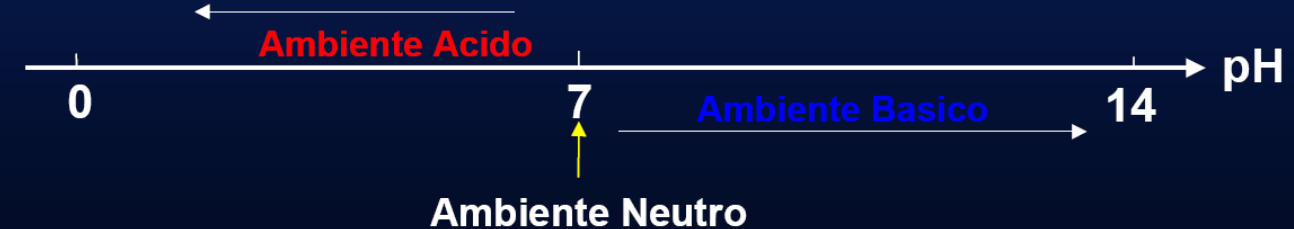
\includegraphics[width=10cm]{immagini/scala_pH.png}
\end{figure}

\subsubsection{Definizioni: pH e P$\boldsymbol{k_a}$}

\subsubsection{Definizioni: pOH e P$\boldsymbol{k_w}$}

\subsubsection{Definizioni: P$\boldsymbol{k_a}$ vs P$\boldsymbol{k_b}$}

\ce{HA <--> H^+ + A^-}

In questa reazione abbiamo un acido che si dissocia in $\rm H^+$ + $\rm A^-$. Correttamente dovremmo scrivere

$$\ce{HA + H_2O <--> H_3O^+ + A^-}$$

Per questa prima specie calcoliamo $k_a$, data da

$$k_a = \left( \rm \frac{[H^+] \cdot [A^-]}{[HA]} \right)$$

Se ad esempio HA fosse l'acido acetico, e anziché metterlo in acqua prendessimo un suo sale come l'acetato di sodio, quest'ultimo, come tutti i sali, si dissocerà totalmente in ioni acetato e ione $\rm Na^+$. Lo ione acetato è la base coniugata dell'acido acetico, in quanto è ottenuto a partire da questo togliendo un protone.

Che succede alla base coniugata di un qualunque acido??

Va da ricordare che se l'acido è debole, la sua base coinugata è forte. Ne segue che la $k_b$ è grande.

\vspace{0.2cm}\ce{A^- + H_2O <--> HA + OH^-}

\vspace{0.2cm}Se mettiamo lo ione $\rm A^-$ (ione acetato nel nostro esempio), questo strappa un protone all'acqua perché è una base forte, formando la specie HA che in teoria è un acido, ma se non si dissocia non manifesta le proprietà acide.

Avendo tolto un protone ad $\rm H_2O$, ci sarà rimasto un eccesso di $\rm OH^-$. Abbiamo quindi scoperto che avevamo messo in acqua un sale neutro e la reazione è basica. Questo perché le basi coniugate degli acidi deboli sono basi forti.

Ciò che succede è che quando mettiamo un sale neutro in acqua questo si dissocia, l'anione poi strappa un protone all'acqua e libera ioni $\rm OH^-$, ottenendo così una soluzione basica.

Ci sarà allora una costante basica, pari a

$$k_b = \left( \rm \frac{[OH^-] \cdot [HA]}{[A^-]} \right)$$

Consideriamo ora il prodotto di $k_a$ e $k_b$

$$k_a \cdot k_b = \left( \rm \frac{[H^+] \cdot [A^-]}{[HA]} \right) \cdot \left( \rm \frac{[OH^-] \cdot [HA]}{[A^-]} \right)$$

$$\implies k_a \cdot k_b = \rm [H^+] \cdot [OH^-] \equiv \textit{k}_\textit{w}$$

Ecco perché se una cresce l'altra diminuisce: perché il loro prodotto deve essere pari a $10^{-14}$ sempre.

Quindi il prodotto della costante di un acido e della costante della sua base coniugata darà sempre il prodotto ionico dell'acqua $k_w$, per cui si avrà sempre che se l'acido è debole la base coniugata sarà forte, mentre se l'acido è forte la sua base coniugata sarà debole.

\vspace{0.2cm}Esempi:
\begin{itemize}
    \item L'aicdo fluoridrico ha costante $k_a=7.2 \cdot 10^{-4}$. La sua base coniugata, lo ione fluoruro $\rm F^-$;
    \item Acido nitroso $\rm HNO_3$ $k_a=4.5 \cdot 10^{-4}$, ione nitrato $\rm NO_3^-$ $k_b=2.2 \cdot 10^{-11}$
    \item Acido solforoso  $k_a=1.2 \cdot 10^{-2}$
\end{itemize}